\section{ŠUM PN PŘECHODU, ŠUM BJT}
Zdroje šumu bipolárního tranzistoru, výpočet výstupního šumu jednoduchého proudového zrcadla

\subsection{Šum PN přechodu}
Šum PN přechodu (diody) je definován pomocí zdroje šumového proudu i\textsubscript{nd}, který je připojen paralelně k dané diodě. i\textsubscript{nd} je závislý na proudu I, který diodou protéká.
\begin{equation}
i_{nd}=\sqrt{2q*I}
\end{equation}

\begin{figure}[h]
   \begin{center}
     \includegraphics[scale=0.5]{images/sumPN.png}
   \end{center}
   \caption{Šum PN přechodu}
\end{figure}

\subsection{Šum BJT}
Šum bipolárního tranzistoru (BJT). BJT tranzistor se vyznačuje třemi šumovými zdroji.
\begin{figure}[h]
   \begin{center}
     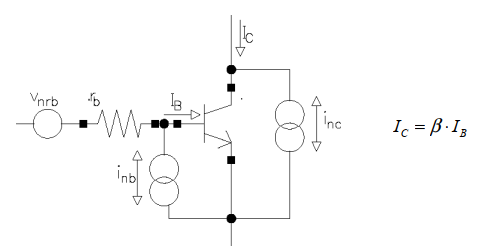
\includegraphics[scale=0.5]{images/sumBJT.png}
   \end{center}
   \caption{Šumové zdroje bipolárního tranzistoru}
\end{figure}
1) Šum odporu báze:
\begin{equation}
v_{nrb}=\sqrt{4kT*r_{b}}
\end{equation}

2) Proudový šum kolektoru
\begin{equation}
i_{nc}=\sqrt{2q*I_{c}}
\end{equation}

3) Proudový šum báze
\begin{equation}
i_{nb}=\sqrt{2q*I_{B}}
\end{equation}

Z praktických důvodů je někdy užitečné převést šumový kolektorový proud i\textsubscript{nc} do myšleného zdroje šumového napětí v\textsubscript{nc} pomocí transkonduktance tranzistoru:
\begin{equation}
g_{m} = I_{c}/U{T}
\end{equation}
\begin{equation}
\Delta I{c} = g_{m}*\Delta U_{BE} => i_{nc} = g_{m} * v_{nc} => v_{nc}=\frac{i_{nc}}{g_{m}}
\end{equation}

\begin{figure}[h]
   \begin{center}
     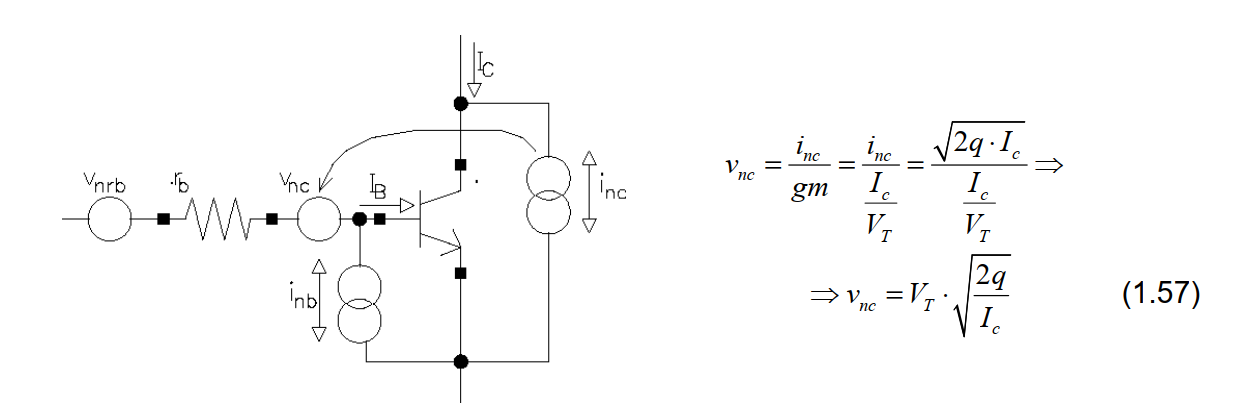
\includegraphics[scale=0.5]{images/prevodBJT.png}
   \end{center}
   \caption{Převod šumového proudu itextsubscript{nc} do vstupního šumového napětí vtextsubscript{nc}}
\end{figure}

Toto přepočítané napětí v\textsubscript{nc} je možné formálně sloučit s šumovým napětím v\textsubscript{nrb} bázového odporu do jediného vstupního šumového zdroje v\textsubscript{ni}:

\begin{figure}[h]
   \begin{center}
     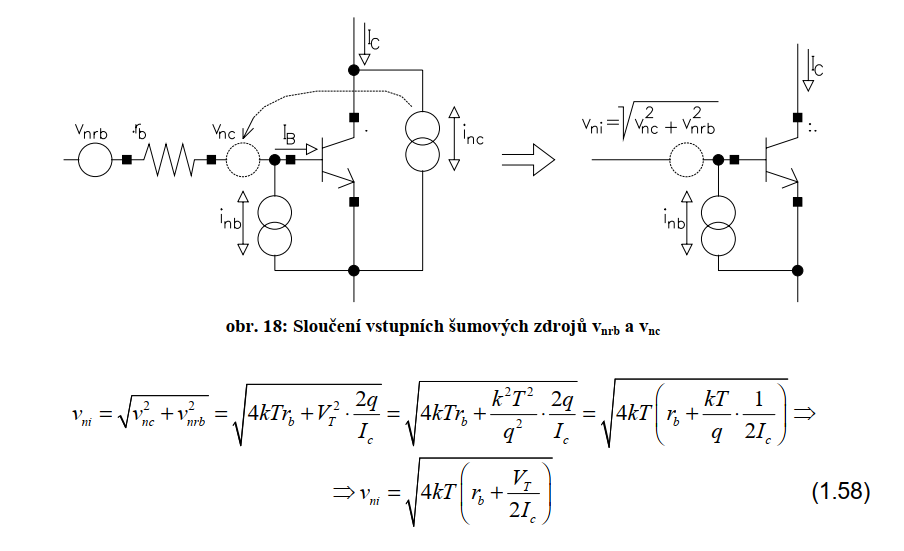
\includegraphics[scale=0.5]{images/slouceniBJT.png}
   \end{center}
   \caption{Sloučení vstupních šumových zdrojů v\textsubscript{nrb} a v\textsubscript{nc}}
\end{figure}

\begin{figure}[h]
   \begin{center}
     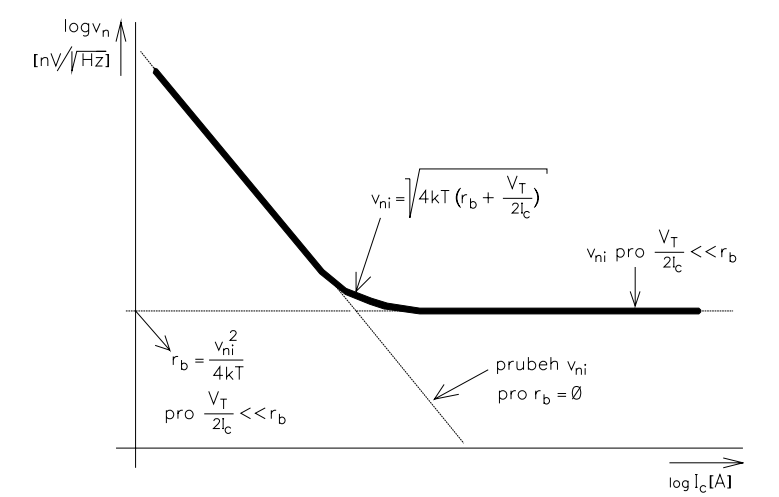
\includegraphics[scale=0.5]{images/grafBJT.png}
   \end{center}
   \caption{ Závislost vstupního šumového napětí BJT tranzistoru na kolektorovém proudu I\textsubscript{c}}
\end{figure}

Kmitočet lomu 1/f šumu (f\textsubscript{k}) je pro NPN tranzistory většinou velmi nízký – i pod 1Hz. Proto jsou NPN tranzistory velmi vhodné pro nízkošumové aplikace určené pro velmi nízké
kmitočty. 

Pro výpočet šumových vlastností základních bloků (proudové zrcadlo, diferenciální stupeň) je někdy výhodné převést šumové napětí bázového odporu do odpovídajícího šumového proudu kolektoru.

\begin{figure}[h]
   \begin{center}
     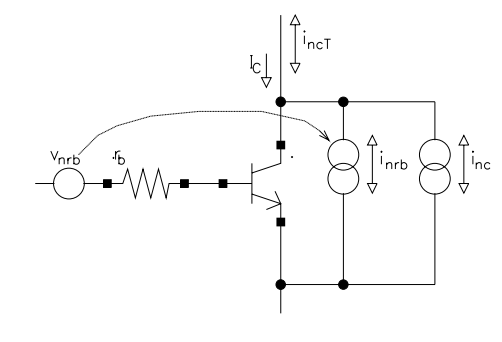
\includegraphics[scale=0.5]{images/nrbBJT.png}
   \end{center}
   \caption{ Převod šumového napětí v\textsubscript{nrb} do šumového proudu i\textsubscript{nrb}}
\end{figure}
\begin{equation}
i_{nc} = \sqrt{2qI_{c}}
\end{equation}
\begin{equation}
i_{nrb} = v_{nrb}*g_{m}=v_{rnb}*\frac{I_{c}}{U_{T}}
\end{equation}
\begin{equation}
i_{nrb} = \sqrt{4*U_{T}*q*r_{b}}*\frac{I_{c}}{U_{T}}=I_{c}*\sqrt{\frac{4*q*r_{b}}{U_{T}}}
\end{equation}

Celkový šumový proud kolektoru i\textsubscript{ncT} je pak:
\begin{equation}
i_{ncT}=\sqrt{2qI_{c}*(1+\frac{2*r_{b}*I_{c}}{U_{T}})}
\end{equation}

\subsection{Výpočet výstupního šumu jednoduchého proudového zrcadla}
\begin{figure}[h]
   \begin{center}
     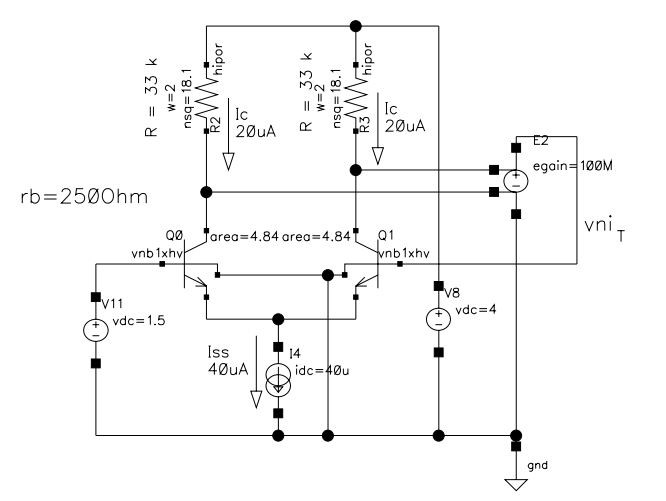
\includegraphics[scale=0.5]{images/symBJT.png}
   \end{center}
   \caption{Symetrický bipolární stupeň s odporovou zátěží}
\end{figure}

Složka vstupního šumu daná NPN tranzistory diferenciálního páru se spočítá jako:
\begin{equation}
v_{ni}=\sqrt{8*k*T*(r_{b}+\frac{U_{T}}{2*I_{c}})}
\end{equation}

Do vstupního šumu se promítá i šum v\textsubscript{nr} zatěžovacích odporů R. Tento šum se na vstup převede tak, že se jeho hodnota podělí ziskem A tohoto diferenciálního stupně. Protože se převádí šum (nekorelovaný) dvou odporů R, je příspěvek odporu roven:
\begin{equation}
v_{nr}*\sqrt{2}
\label{eqn:vnr}
\end{equation}
Poté tedy:
\begin{equation}
v_{nr}*\sqrt{2}=\sqrt{8*k*T*R}=\sqrt{8*U_{T}*q*R}
\end{equation}
\begin{equation}
A=g_{m}*R=\frac{I_{ss}*R}{U_{T}}
\end{equation}
Šum z rovnice \ref{eqn:vnr} obou odporů R je převeden na svtupní složku v\textsubscript{nri}:
\begin{equation}
v_{nri}=\frac{v+{nr}*\sqrt{2}}{A}=4*U_{T}*\sqrt{\frac{2*k*T}{R*I_{ss}^2}}
\end{equation}
Celkové vstupní šumové napětí v\textsubscript{niT} se potom spočítá jako nekorelovaný součet složek v\textsubscript{nri} a v\textsubscript{ni}:
\begin{equation}
v_{niT}=\sqrt{v_{nr}^2+v_{ni}^2}
\end{equation}




























